% !TEX root = 99_main.tex

Cozie is built as a clock-face for fitbit, a wearable health tracker with 25 million active users \cite{fibit2018}. The application is publicly available for download at the following link [insert link]

\subsection{Overview}

In this section we define "user" as the test participant who is wearing the fitbit, and "manager" as the person coordinating the experiment. \ 

The default status of the clock-face is a simple binary question: "Comfy" or "Not Comfy", as seen in Figure \ref{fig:homescreen}. By simply clicking one of the icons, information about the users location (GPS), heart-rate, steps walked since last log, and the comfort data is anonymously sent to an Influx time series cloud database [Ref influx]. Data from this database can be simply queried with an API key that can be provided to the manager. Further documentation can be found on the cozie website [insert link].\\

If the manager is interested as to why the user is feeling discomfort, then there is a range of additional questions that can be configured using the cellphone that the fitbit is paired with. The optional questions include:

\begin{itemize}
  \item Thermal: Prefer Warmer - Prefer Cooler
  \item Light: Prefer brighter - Prefer Dimmer
  \item Noise: Prefer Louder - Prefer Quieter 
  \item Mood: Good - Neutral - Not So Good
  \item Location: Indoor - Outdoor
  \item Location: In Office - Out of Office
\end{itemize}

These responses will be grouped with the afore mentioned data, and stored in the Influx time series database. The manager is invited to contact the authors if they have further tailored questions that they would like to add.\\

A unique user-id for each user, and a unique experiment-id can be configured by the manager using the cellphone that the fitbit is paired with. \\

The watch-face also has the ability to prompt the user with a 3 second vibration, and force them to provide comfort feedback. This may be triggered at certain hours of the day, random hours of the day, at set time intervals, or at each 1000 steps walked. 


\begin{figure}
\begin{center}
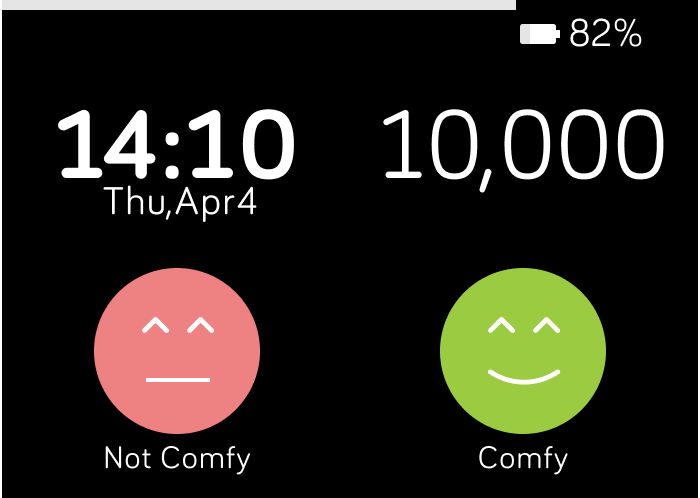
\includegraphics[width=0.2\textwidth, trim= 0cm 0cm 0cm 0cm,clip]{homescreen.png}
\caption{Homescreen}
\label{fig:homescreen}
\end{center}
\end{figure}

% \subsection{Building Data Labeling}

% The human comfort feedback can be combined with building sensor data to create a labeled data set of the environment. (perhaps talk more or delete this section)

% An example of this in practice will be introduced in the next section.